\chapter{Tecnologie utilizzate}
\label{chap:2}

\section{Introduzione alle tecnologie}
\label{sec:IntroduzioneTecnologie}
Come già introdotto brevemente nel capitolo \ref{chap:1}, per lo scopo di questa tesi si è scelto di confrontare due approcci differenti, ma sempre più utilizzati nelle applicazioni web moderne.
In particolare si partirà da WebAssembly e dall'interfaccia di sistema WASI, per finire con un'introduzione anche su Node.js.

\section{WebAssembly}
\label{sec:Wasm}
WebAssembly (Wasm) è uno standard che definisce un formato binario (.wasm) e un relativo formato testuale (.wat) per la scrittura di codice eseguibile nelle pagine web. 
Wasm è attualmente sviluppato in maniera open-source, da un \emph{Community Group} del W3C che comprende membri di tutti i browser più utilizzati.
\\Esso è nato principalmente come integrazione a JavaScript, per consentire l'esecuzione di codice ad una velocità paragonabile a quella del codice nativo, grazie alla dimensione ridotta dei file binari generati e alla loro efficienza.
\\Inoltre grazie all'esecuzione all'interno di una sandbox è garantita un ottima sicurezza, anche sotto il punto di vista della memoria.
\\Grazie al formato testuale (.wat), è possbile eseguire debug, test, ottimizzazioni, scrivere a mano programmi di basso livello, ma anche visualizzare i sorgenti dei moduli wasm, quando questi sono utilizzati una pagina web.
\cite*{wasmDesign}
\\Al giorno d'oggi è in costante crescita, sia il numero di linguaggi che possono avere come \emph{compilation target} WebAssembly (Rust, C, Go, Kotiln, etc), sia il numero di siti che sfruttano tale tecnologia, grazie anche al fatto che praticamente ogni browser attualmente utilizzato, supporta Wasm. 
\begin{figure}
        \begin{center}
                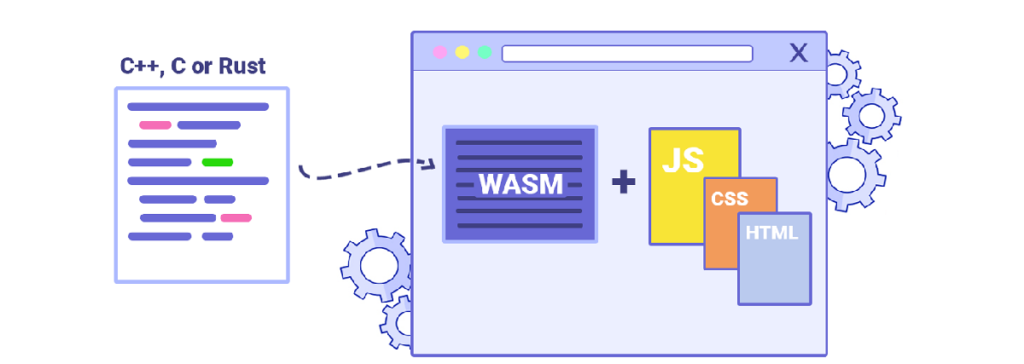
\includegraphics[width=0.8\columnwidth]{images/wasm.png}
        \end{center}
        \caption{WebAssembly all'interno del browser}
        \label{fig:wasm}
\end{figure}
\subsection{Storia e Origini}
\subsubsection{I predecessori}
Nel 2011 Google rilasciò un progetto open source chiamato \textbf{Native Client (NaCl)}.
L'obiettivo era quello di consentire l'esecuzione di codice nativo nel browser all'interno di una sandbox con privilegi limitati.
In particolare si stava cercando di supportare software che richiedevano grande sforzo computazionale (simulazioni, elaborazioni di audio e video e giochi).
\\Il progetto si rivelò un successo sotto il punto di vista prestazionale. Vennero infatti rilasciati diversi software e giochi che presentavano prestazioni simili alla rispettiva versione Desktop.
Non mancavano però diversi problemi. Il codice ottenuto era eseguibile solo nel browser Chrome ed era impossibile l'interazione con JavaScript o con altre API sul web.
\\Un tentativo di evoluzione fu presentato nel 2013 dal team di Mozilla. Si trattava di \textbf{asm.js}, un sottoinsieme di JavaScript che consentiva l'invocazione di funzioni scritte in linguaggi come C, C++ o Rust, in diversi browser e direttamente da JavaScript.
A discapito di una maggior portabilità ci fu una significativa diminuizione delle prestazioni, dovuta alla lentezza dell'interprete JavaScript, che era stato caricato di un notevole overhead.
\\Queste due soluzioni dimostrarono la possbilità di eseguire codice in una sandbox, o con ottime prestazioni, ma solo all'interno di Chrome (NaCl), oppure in diversi browser ma con prestazioni decisamente inferiori.
Si voleva quindi trovare un modo per unificare gli enormi vantaggi offerti da ognuno dei due approcci.\cite*{wasmBook}
\subsubsection{La nascita di Wasm}
Fu nel Giugno 2015 che Brendan Eich (creatore di JavaScript), insieme ad altri sviluppatori di Mozilla, annunciarono che lo sviluppo di WebAssembly era cominciato.\cite*{asmjsToWasm}
Wasm venne presentato come "un nuovo standard open source che definiva un formato e un modello di esecuzione portabile, efficiente in termini di dimensioni e tempo di caricamento, specificamente progettato per essere un target di compilazione per il web".
WebAssembly prometteva prestazioni fino a 20 volte superiori rispetto ad asm.js, grazie alla maggiore velocità di decodifica dei file binari rispetto a quella di parsing da parte dell'interprete JavaScript per i file di asm.js.
Nel 2017 venne lanciato il \emph{minimum viable product} (MVP), che conteneva pressochè le stesse funzionalità presenti in asm.js e venne dichiarata conclusa la fase di preview.
Capendo le potenzialità di ciò che stava venendo sviluppato hanno dato il loro contributo al progetto, aziende del calibro di Google, Microsoft, Apple, Unity.

\subsection{Casi d'uso}
Inizialmente ci si è concentrati sull'utilizzo di WebAssembly all'interno del browser e venivano presentati svariati casi d'uso:
\begin{itemize}
        \item Elaborazione di immagini e video;
        \item Giochi;
        \item Applicazioni peer-to-peer;
        \item Applicazioni CAD;
        \item Realtà virtuale e realtà aumentata con latenza minima;
        \item Riconoscimento di immagini;
        \item Simulazione/emulazioni di sistemi operativi (QEMU, DOSBox);
        \item Applicazioni per desktop ridimensionamento;
        \item Web server locali;
\end{itemize}
Si era pensato fin da subito anche alla portabilità ed erano stati presentati diversi possibili utilizzi anche per ambienti non-web:
\begin{itemize}
        \item Esecuzione server-side di codice non attendibile;
        \item Servizi per la distribuzione di giochi;
        \item Generiche applicazioni server side;
        \item Calcolo simmetrico, distribuito su più nodi;
\end{itemize}
\subsection{Concetti chiave}
WebAssembly codifica un linguaggio di programmazione di basso livello, simile ad Assembly. Tale linguaggio è strutturato attorno ai seguenti concetti:\cite*{wasmSpec}

\subsubsection{Valori}
In WebAssembly sono presenti:
\begin{itemize}
        \item Un tipo \emph{byte} per la rappresentazione di byte non interpretati;
        \item Quattro tipi di valori numerici: interi e numeri a virgola mobile, ognuno da 32 o 64 bit (\emph{i32, i64, f32, f64});
        \item Un tipo vector a 128 bit(\emph{i128}) contenente anch'esso valori numerici (ad esempio da 2 f64, oppure da 4 i32 etc.);
        \item Un tipo riferimento per puntatori a differenti entità;
\end{itemize}
Quest'ultimo è definito "opaco", in quanto non è visibile né la loro dimensione, né la loro rappresentazione in bit. Al contrario i primi due tipi si dicono "trasparenti".
\\Infine è anche possibile .
\subsubsection{Istruzioni}
Il modello computazionale di WebAssembly è basato su uno stack. Il codice è costituito da una sequenza di istruzioni eseguite in ordine. Le istruzioni sfruttano una struttura dati detta \emph{operand stack} e possono essere di tipo semplice, o di controllo.
\\Le operazioni semplici svolgono manipolazioni basilari sui dati, prelevando parametri dallo stack (\emph{pop}) e inserendo il risultato nello stesso (\emph{push}). Le operazioni di controllo, si occupano invece di alterare il flusso di esecuzione grazie a costrutti condizionali, blocchi e cicli.
\subsubsection{Traps} 
Alcune istruzioni possono fallire e generare degli errori (traps) che non è possibile gestire all'interno di WebAssembly. Tali errori vengono infatti lanciati nell'ambiente di esecuzione dell'host dove, al contrario, vengono normalmente gestiti.
\subsubsection{Funzioni}
Il codice è diviso in funzioni. Ognuna di queste ha una certe sequenza di valori sia come parametri che come tipo di ritorno. In una funzione viene eseguita una serie di istruzioni, possono inoltre essere chiamate altre funzioni (anche ricorsivamente) e create variabili locali.
\subsubsection{Tabelle}
Una tabella è un array di valori "opachi" di un particolare tipo. Tale struttura consente al programma di ottenere i valori indirettamente attraverso un indice dinamico. Tramite le tabelle è possibile, per esempio invocare funzioni indirettamente, emulando in questo modo i puntatori a funzione.
\subsubsection{Memoria lineare}
La memoria lineare è un  array continuo di byte. Ha una dimensione iniziale che può crescere dinamicamente al bisogno. Un programma può leggere e scrivere valore in memoria (operazioni di \emph{load/store}) in un qualsiasi indirizzo al suo interno (anche in maniera non allineata).
\subsubsection{Moduli}
Un modulo è l'unità di deployment per un programma WebAssembly. Esso conterrà le definizioni di funzioni, tabelle, memoria etc. In un modulo è anche possibile esportare o importare definizioni, inizializzare tabelle o memoria lineare e anche definire una funzione \emph{start} che verrà eseguita automaticamente. 
\subsubsection{Embedder}
Solitamente un modulo WebAssembly sarà integrato in un host che ne definirà l'inizializzazione, la risoluzione delle funzioni importate  e le modalità di accesso di quelle esportate. L'Embedder è l'entità che implementa la connessione tra l'ambiente host e il modulo Wasm. Ci si aspetta che l'embedder interagisca con la semantica di WebAssembly in un modo ben definito nelle specifiche del formato Wasm.
\begin{figure}
        \begin{center}
                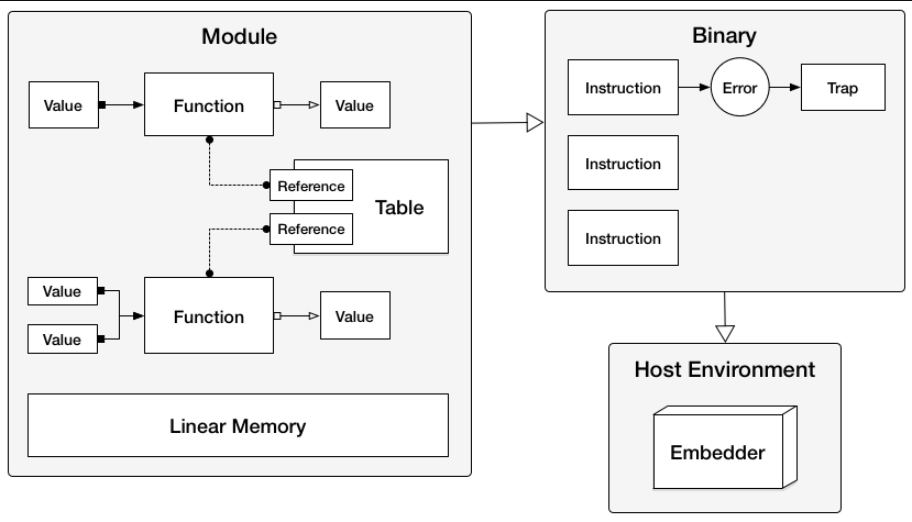
\includegraphics[width=0.9\columnwidth]{images/wasmArchitecture.png}
        \end{center}
        \caption{Architettura di WebAssembly}
        \label{fig:wasmArch}
\end{figure}
\newpage
\subsection{Fasi semantiche}
Nella semantica di WebAssembly è possibile individuare tre fasi principali: decodifica, validazione ed esecuzione.\cite*{wasmSpec}
\subsubsection{Decodifica}
I moduli WebAssembly sono distribuiti in formato binario (.wasm) e per questo è necessario decodificarli in modo da ottenere una rappresentazione interna del modulo, con cui il web browser o il runtime environment potrà lavorare.
\subsubsection{Validazione}
Dopo aver decodificato i moduli binari, per poterli istanziare, è necessario controllare che questi siano validi.
La validità è verificata grazie ad un sistema di tipi basato sulla sintassi astratta di un modulo e sul suo contenuto. In particolare per ogni componente della sintassi è presente una regola che specifica le condizioni da rispettare perchè il modulo risulti valido.
\begin{figure}
        \begin{center}
                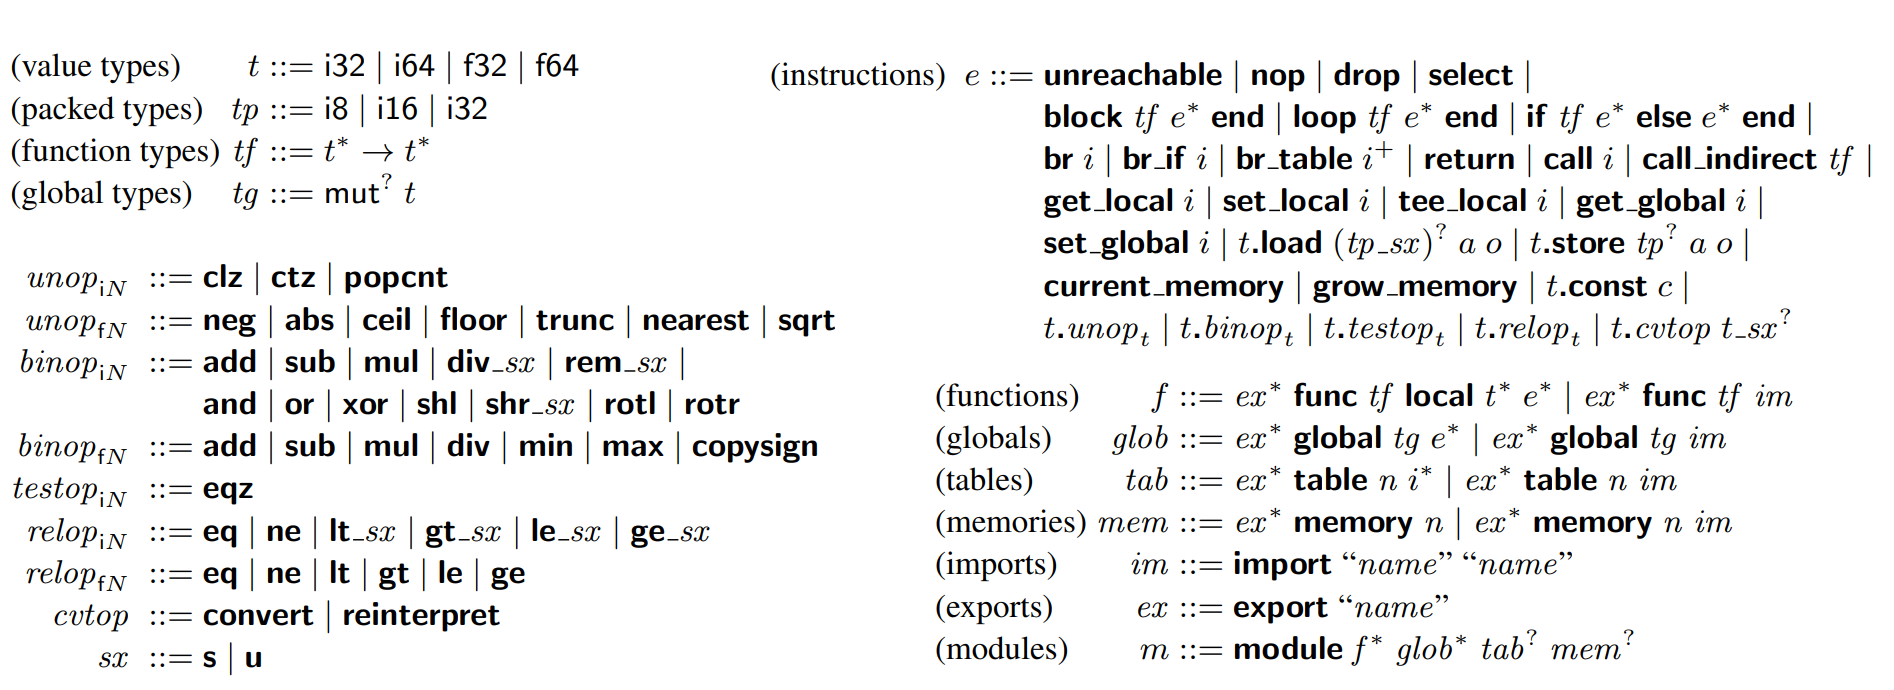
\includegraphics[width=1\columnwidth]{images/wasmSyntax.png}
        \end{center}
        \caption{La sintassi astratta di WebAssembly}
        \label{fig:wasmSyntax}
\end{figure}
\\Ad esempio viene controllato l'ordine delle istruzioni nel corpo di una funzione assicurandosi che lo stack sia utilizzato nel modo corretto.
Oppure se nelle specifiche esaminiamo un'operazione binaria tra tipi numerici (i32.add, f64.xor etc.), notiamo che essa è del tipo \emph{t.binop} e dato un contesto \(C\) essa è valida solamente con tipo \([t~t]{\rightarrow} [t]\).
\\Tale regola si può anche rappresentare con la seguente notazione formale:
\begin{equation*}
\frac{
}{
        C {\vdash} t\mathsf{.}{\mathit{binop}} : [t~t] {\rightarrow} [t]
}
\end{equation*}
Esaminando invece le regole di validazione di un'istruzione per l'aumento di memoria lineare \emph{memory.grow} (tale istruzione si aspetta l'offset che indica di quanto la memoria è da espandere e ritorna la dimensione della memoria precedente all'espansione) notiamo che:
\begin{itemize}
        \item La memoria \(C.{\mathit{mems}}[0]\) deve essere definita nel contesto;
        \item Allora l'istruzione risulta valida con tipo \([{\mathit{i32}}] {\rightarrow} [{\mathit{i32}}]\);
\end{itemize}
In notazione formale:
\begin{equation*}
        \frac{
        C.{\mathit{mems}}[0] = {\mathit{memtype}}
      }{
        C {\vdash} {\mathit{memory.grow}} : [{\mathit{i32}}] {\rightarrow} [{\mathit{i32}}]
      }        
\end{equation*}
\subsubsection{Esecuzione}
Terminata la validazione di ogni istruzione il modulo può finalmente essere istanziato.
L'istanza di un modulo ne è la rappresentazione dinamica. Esso comprende lo stack, sul quale operano le istruzioni WebAssembly e uno \emph{\textbf{store}} astratto, contenente lo stato globale (è la rappresentazione a runtime di tutte le istanze di funzioni, tabelle, memorie etc. che sono state allocate dall'istanziazione).
Terminata l'istanziazione, diventa effettivamente possibile l'esecuzione di istruzioni WebAssembly.
\\In particolare, se nel modulo era stata definita una funzione \emph{\_start}, essa sarà eseguita subito dopo la creazione dell'istanza, altrimenti sarà possibile invocare funzioni esportate, chiamandole direttamente dall'istanza stessa.
\\Per ogni istruzione, è presente una regola che specifica l'effetto della sua esecuzione sullo stato del programma. Rimanendo coerenti con gli esempi sulla validazione, segue il comportamento dell'istruzione \emph{t.binop}:

\begin{itemize}
        \item In seguito alla validazione, possiamo assumere che due valori di tipo \(t\) si trovino in cima allo stack;
        \item Viene eseguita l'operazione di \textbf{pop} del valore \(t.const~c_1\) dallo stack;
        \item Viene eseguita l'operazione di \textbf{pop} del valore \(t.const~c_2\) dallo stack;
        \item Se \({\mathit{binop}}_t(c_1, c_2)\) è definita allora:
        \begin{itemize}
                \item Sia \(c\) il possibile risultato di \({\mathit{binop}}_t(c_1, c_2)\);
                \item Viene eseguita l'operazione di \textbf{push} del valore \(t.const~c\) nello stack.
        \end{itemize}
        \item Altrimenti:
        \begin{itemize}
                \item Trap.
        \end{itemize}
\end{itemize}
In notazione formale:
\begin{equation*}
        \begin{split}\begin{array}{lcl@{\qquad}l}
                (t\mathsf{.}{\mathsf{const}}~c_1)~(t\mathsf{.}{\mathsf{const}}~c_2)~t\mathsf{.}{\mathit{binop}} &{\hookrightarrow}& (t\mathsf{.}{\mathsf{const}}~c)
                  & (\mathrel{\mbox{if}} c \in {\mathit{binop}}_t(c_1,c_2)) \\
                (t\mathsf{.}{\mathsf{const}}~c_1)~(t\mathsf{.}{\mathsf{const}}~c_2)~t\mathsf{.}{\mathit{binop}} &{\hookrightarrow}& {\mathsf{trap}}
                  & (\mathrel{\mbox{if}} {\mathit{binop}}_{t}(c_1,c_2) = \{\})
                \end{array}\end{split}
\end{equation*}
Non viene riportato l'esempio anche sull'istruzione \emph{memory.grow} essendo una funzionalità decisamente più complessa (11 diversi passaggi, con svariati sottocasi) che comporterebbe obbligatoriamente, l'introduzione di ulteriori dettagli che esulano dallo scopo di questa tesi.
\break
Si noti che sia l'istanziazione, che l'invocazione di funzioni, sono operazioni che avvengono all'interno dell'ambiente di esecuzione dell'host.
\begin{figure}
        \begin{center}
                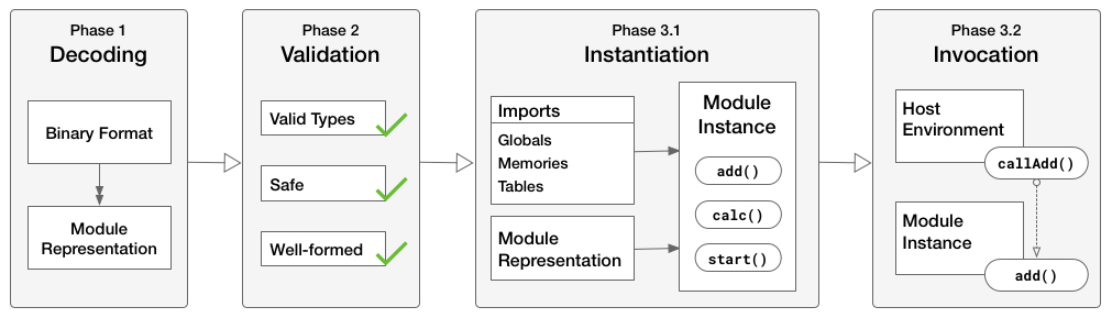
\includegraphics[width=0.97\columnwidth]{images/wasmSemanticPhases.png}
        \end{center}
        \caption{La semantica di WebAssembly}
        \label{fig:wasmPhases}
\end{figure}

\newpage
\subsection{Correttezza logica}
Grazie alla sua semantica è possibile dire che il sistema di tipi di WebAssembly è logicamente corretto (\emph{sound})\cite*{wasm:soundness}. Esso infatti garantisce sia \emph{\textbf{type safety}}, che \emph{\textbf{memory safety}}.
\\Per quanto riguarda la sicurezza rispetto ai tipi, tutti i tipi controllati durante la validazione saranno rispettati anche a runtime:
\begin{itemize}
        \item Ogni variabile (locale o globale) conterrà valori del tipo corretto.
        \item Ogni istruzione verrà applicata solo ad operandi del tipo che ci si aspetta e restituirà valori del tipo corretto.
        \item Ogni funzione restituirà valori del tipo previsto, a meno di errori (trap).
\end{itemize}
Per quanto riguarda la \emph{memory safety}, è garantito che non verrà acceduta nesun'area di memoria, diversa da quelle esplicitamente specificate dal programma. Ogni volta che per esempio verrà fatta un'operazione di load/store in un certo indirizzo di memoria, si controllerà che quest'ultimo sia nel range di indirizzi possibili per l'istanza attuale di WebAssembly.
\\Inoltre sono garantite altre proprietà: 
\begin{itemize}
        \item L'assenza di comportamenti indefiniti: le regole di esecuzione sono mutualmente consistenti e coprono qualsiasi caso che possa capitare in un programma validato.
        \item L'incapsulamento per funzioni e moduli: nessuna variabile locale può essere acceduta fuori dalla funzione dove è dichiarata e nessun componente di un modulo può essere acceduto fuori dallo stesso a meno che quest'ultimo non sia esportato o importato.
\end{itemize}
Infine è importante notare che le regole di validazione si occupano solamente dei componenti statici di un programma WebAssembly. Per dimostrare correttezza in maniera precisa, sono state estese le \emph{typing rules} anche ai componenti dinamici, come lo \textbf{store}, le \textbf{configurations} (coppie Store - Thread di esecuzione) e le istruzioni amministrative.
Dopo aver dato la definizioni di configurazione valida è stato possibile enunciare due teoremi e derivare un corollario che riassumendo dicono che:
\\Ogni thread in una \emph{configuration} valida o esegue per sempre, o termina con un errore (trap), o termina con un risultato del tipo atteso. Di conseguenza, dato uno \emph{store} valido, nessun calcolo derivante dall'istanzazione o dall'invocazione di un modulo valido, può avere comportamenti diversi da quelli definiti nelle specifiche. \cite*{wasm:soundness:theorems}
\subsection{Creazione e utilizzo di moduli WebAssembly}
Sebbene sia possibile scrivere a mano il codice dei moduli WebAssembly, è molto più comune scrivere il codice in un linguaggio di alto livello e poi compilare quest'ultimo in un modulo Wasm.
Nonostante durante lo sviluppo iniziale del linguaggio ci si fosse concentrati solo sull'utilizzo di C/C++, ad oggi sono più di 10 i linguaggi che supportano WebAssembly come \emph{compilation target}. Tra questi spiccano Rust, C\#, Python, Kotlin, Swift, Go. 
\\Per esempio, utilizzando Rust sarebbe sufficiente scrivere un normale programma e poi lanciare il seguente comando nella directory del progetto: 
\begin{lstlisting}[language=Bash, numbers=none, label=lst:RustCompile, caption={}]
wasm-pack build
\end{lstlisting}
Tale comando compilerà il programma in un modulo WebAssembly, generando un file \textbf{.wasm} utilizzabile dal codice JavaScript della nostra pagina web.
\\Bisogna però sottolineare che sin dagli albori di WebAssembly, non era mai stata fatta nessuna assunzione sull'ambiente host e che il utilizzo non sarebbe stato limitato alle sole pagine web.
\\In particolare, per lo scopo di questa tesi, sarà necessario che i moduli WebAssembly vengano istanziati ed eseguiti server side, ma soprattuto che tali moduli abbiano accesso al \textbf{file system} e a funzioni di \textbf{I/O}.
Tali funzioni in WebAssembly non sono disponibili, a causa dell'esecuzione all'interno di una sandbox e delle caratteristiche di sicurezza. Per questi e per molti altri motivi è stato sviluppato WASI (WebAssembly System Interface).
\newpage
\section{WebAssembly System Interface}
\label{sec:WASI}
WebAssembly System Interface è una famiglia di API progettate dai membri della Bytecode Alliance durante lo sviluppo del progetto \textbf{Wasmtime}.\cite*{wasiHome}
\\WASI si propone di standardizzare l'accesso a varie funzionalità tipicamente associate ai sistemi operativi, da parte di programmi scritti in WebAssembly. In particolare lo sviluppo è partito da una serie di funzioni basiche simili a quelle contenute in POSIX.
D'ora in avanti queste funzioni verranno spesso menzionate come \textbf{syscall}, in quanto esse hanno uno scopo simile o analogo a quello delle system call in programmi eseguibili nativi.
Bisogna però tenere a mente che tali "syscall" sono semplicemente una serie di funzioni che permettono di eseguire operazioni di I/O. Ne sono un esempio:
\begin{itemize}
        \item Accesso a file e File System;
        \item Funzioni per le socket di Berkeley;
        \item Funzionalità relative al tempo e ai numeri random;
\end{itemize}
WASI è progettato in modo da essere indipendente dai browser e da non dipendere da JavaScript o da API web. Inoltre non è limitato dal bisogno di essere compatibile con JavaScript ed ha integrato un sistema di sicurezza \emph{capability based} che consente di estendere le caratteristiche di sandboxing presenti in WebAssembly, rendendo possibile l'I/O.
\\Attualmente WASI ha attraversato due fasi di preview (preview0, preview1), le quali dovrebbero essere seguite da due ulteriori preview e infine dalla prima release ufficiale (WASI 1.0).
\subsection{Gli obiettivi}
WASI è nato con una serie di obiettivi di alto livello, che si ispirano e integrano gli obiettivi di WebAssembly.\cite*{wasi:goals} Esso si propone di:
\begin{itemize}
        \item Creare un insieme di API progettate direttamente per programmi WebAssembly. Esse devono essere portabili (utilizzabili su diversi sitemi), modulari (composte da più componenti riutilizzabili), indipendenti dal runtime sottostante e devono mantenere la caratteristiche di sicurezza garantite da WebAssembly (sandbox) grazie ad un progettazione basata su \textbf{Capabilties};
        \item Sviluppare e implementare funzionalità in maniera incrementale. Inizialmente si ha un Minimum Viable Product (MVP) che include funzionalità essenziali, che verrà gradualmente espanso aggiungendo nuove feature sulla base di feedback ed esperienze pratiche;
        \item Arricchire la progettazione delle API con documentazione e test completi e quando possibile, fornire anche implementazioni di riferimento condivisibili tra diversi runtime Wasm;
        \item Lavorare al fianco degli sviluppatori di strumenti e librerie Wasm in modo da garantire ai loro utenti anche il supporto per WASI;
        \item Consentire alle proprie API di evolvere nel tempo. Ciò significa anche consentire l'evoluzione di moduli standardizzati e l'introduzione di nuovi moduli. Per garantire compatibilità possono essere create implementazioni dei moduli standardizzati, utilizzando librerie basate su nuove API, consentendo in questo modo una transizione fluida mentre la piattaforma;
\end{itemize}
\subsection{I principi di design}
WebAssembly System Interface è tutt'ora in fase di sviluppo secondo una serie di \emph{\textbf{design principle}} che verranno illustrati di seguito:\cite*{wasi:designPrinciples}
\subsubsection{Capability}
WASI segue un concetto di sicurezza basata su capability che era già stata presentata qualche anno prima da CloudABI's.
\\File, directory, socket e altre risorse sono identificati da indici interi (paragonabili ai file descriptor utilizzati nei sistemi UNIX), contenuti in tabelle esterne che rappresentano le capabilties per un certo modulo WASI.
Le API di WASI potranno quindi accedere ed utilizzare una risorsa, solo se a questa è associata una deterrminata capability.
Ad esempio, per l'apertura di un file WASI mette a disposizione una system call simile alla \textbf{openat}.
Essa si aspetta che il processo chiamante abbia il file descriptor della directory contenente tale file, il quale rappresenterà la capability per l'apertura dei file all'interno di quella specifica directory.
\\In realtà è anche possibile un approccio più simile alla classica system call "open".
Infatti, grazie alla pre-apertura di una directory al lancio del programma essa verrà inclusa nella tabella delle capabilties, la quale verrà automaticamente controllata a runtime ogni volta che il programma invocherà la "open".
\\Tutto ciò è simile a ciò che avviene normalmente in POSIX, con la differenza che POSIX normalmente consente ad un processo di richiedere qualsiasi file descriptor nell'intero file system e poi l'accesso sarà concesso a seconda delle policy di sistema, mentre in WASI è necessario che un programma abbia le capability giuste per accedere alle risorse di una certa directory. In questo modo diventa possbile l'esecuzione di codice non attendibile, dando permessi per specifiche directory a runtime, senza la necessità di impostare permessi nel file system.\cite*{wasi:capabilities}
\subsubsection{Interposizione}
L'interposizione è la capacità di un'istanza di WebAssembly di implementare un'interfaccia WASI che poi potrà essere utilizzata in maniera trasparente da un'altra istanza (consumer).
Ciò può essere sfruttato per adattare o attenuare le funzionalità di un API WASI, senza cambiare il codice che la utilizza.
Tale concetto viene anche spesso chiamato "virtualizzazione".
\subsubsection{Compatibilità}
La compatibilità con applicazioni e host diversi è un obiettivo primario di WASI. Certe volte però è possibile che essa sia in confliatto con una progettazione chiara delle API, oppure con la sicurezza, le performance o la portabilità.
Perciò si è cercato di appesantire il meno possibile le API di WASI con aspetti riguardanti la compatibilità e di garantire questo tema grazie all'utilizzo di librerie. Ne è un esempio WASI-libc, libreria costruita on top alle system call di WASI che fornisce una grande varietà di API compatibili con posix (standard I/O, file I/O, gestione della memoria, stringhe etc.).
In questo modo applicazioni che non hanno bisogno di particolari funzionalità di compatibilità, non verranno appesantite da complessità non necessaria.
\subsubsection{Portabilità}
La possibilità di eseguire codice in maniera consistente ed efficace in runtime environment o su piattaforme differenti è molto importante nel contesto di WASI. Bisogna però sottolineare che il significato di portabilità potrebbe variare molto da un API all'altra. Come già introdotto precedentemente WASI nasce come una tecnologia modulare e non necessariamente ogni sua API dovrà essere implementata da ogni WebAssembly Engine.
La decisione è stata quella di non escludere un API solo perchè alcune tipologie di host non sarebbero in grado di implementarla totalmente.
\\In ogni caso verranno preferite API che possano essere eseguite in più ambienti possibili, ma la valutazione su cosa sia sufficientemente portabile e cosa no, verrà effettuata caso per caso.
\subsubsection{Modularità}
WASI è progettato per offrire svariate interfacce ed è pressochè impossibile che tutte siano appropriate per tutti gli \emph{host environment}. Per questo motivo WASI utilizza un approccio a componenti che consente di descrivere quali API siano adatte per un certo ambiente e quali no. In quaesto modo ci si assicurà che un programma avrà accesso solamente alle interfacce che sono rilevanti per un dato environment.
\subsection{Esempi}
Per capire meglio che cos'è realmente una system call WASI seguono una serie di esempi riguardanti funzioni che saranno poi invocate anche dal modulo scritto per il prototipo di questa tesi.\cite*{wasi:api}
Si parte esaminando la funzione \textbf{path\_open} che consente l'apertura di un file o directory.
\\\textbf{path\_open(fd: fd, dirflags: lookupflags, path: string, oflags: oflags, fs\_rights\_base: rights, fs\_rights\_inheriting: rights, fdflags: fdflags) -> Result<fd, errno>}
\\\textbf{Parametri}:
\begin{itemize}
        \item fd: \textbf{fd};
        \item dirflags: \textbf{lookupflags} Flag che indica il metodo di risoluzione del path (se il path è un link simbolico esso verrà espanso);
        \item path: \textbf{string};
        \item oflags: \textbf{oflags} Flag booleani per indicare il metodo di apertura (creat, directory, excl, trunc);
        \item fs\_rights\_base: \textbf{rights} Permessi iniziali del file descriptor appena creato. Sono permessi che si applicano esclusivamente ad operazioni fatte usando il file descriptor stesso. Può capitare che l'implementazione restituisca un file descriptor con permessi più restrittivi di quelli specificati, se tali permessi non sono applicabili al tipo di file aperto;
        \item fs\_rights\_inheriting: \textbf{rights} Permessi che si applicano a file descriptor derivati da quello iniziale;
        \item fdflags: \textbf{fdflags} Flag per il file descriptor restituito (append, dsync, noblock, rsync, sync);
\end{itemize}
\textbf{Risultato}:
\begin{itemize}
        \item ok: \textbf{fd} 
        \item err: \textbf{errno} Codice errore restituito da una funzione (noent, perm, notsock etc.)
\end{itemize}
Per capire meglio il funzionamento delle capability, si citano alcuni permessi (\textbf{rights}) applicabili a un file descriptor:
\begin{itemize}
        \item fd\_read: \textbf{bool} Permesso di invocare \textbf{fd\_read} e \textbf{sock\_recv}
        \item fd\_write: \textbf{bool} Permesso di invocare \textbf{fd\_write} e \textbf{sock\_send}
        \item path\_create\_directory: \textbf{bool} Permesso di invocare \textbf{path\_create\_directory}
        \item sock\_accept: \textbf{bool} Permesso di invocare \textbf{sock\_accept} 
\end{itemize}
Si procede esaminare la funzione \textbf{fd\_read}, simile alla \textbf{readv} di POSIX.
\\\textbf{fd\_read(fd: fd, iovs: iovec\_array) -> Result<size, errno>}
\\\textbf{Parametri}:
\begin{itemize}
        \item fd: \textbf{fd} File descriptor del file che è stao aperto;
        \item iovs: \textbf{iovec\_array)} Lista di \emph{scatter/gather vector} in cui contenere i dati letti;
\end{itemize}
\textbf{Risultato}:
\begin{itemize}
        \item ok: \textbf{size} Numero di byte letti.
        \item err: \textbf{errno} Codice errore restituito da una funzione (noent, perm, notsock etc.)
\end{itemize}
\subsection{Wasmtime}
Per lo scopo di questa tesi è necessaria l'esecuzione di un modulo WebAssembly, che sfrutti anche API di WASI, all'interno di un server sviluppato nel linguaggio di programmazione Rust.
Al momento le soluzioni possbili per un embedding di questo tipo, sono diverse (Wasmtime, Wasmer), ma non così numerose.
Tra queste si è optato per Wasmtime, un progetto sviluppato della Bytecode Alliance.
\\Wasmtime è un runtime environment standalone, ottimizzato per WebAssembly e WASI.
Permette di eseguire codice WebAssembly all'esterno del browser in applicazioni di qualsiasi grandezza e scritte in molteplici linguaggi differenti (Rust, C, Python, Go, Ruby, Bash etc.).
Proprio come in WebAssembly, un'obiettivo di Wasmtime è quello di eseguire codice non attendibile in sicurezza all'interno di una sandbox.
Inoltre Wasmtime implementa le API di WASI per l'accesso al file system, in modo che un programma possa accedere solo ai file e alle directory per i quali ha le capability.
\cite*{wasmtime}
\newpage
\subsection{Struttura di WASI}
\subsection{Wasmtime}
\subsection{Applicazioni e Casistiche d'Uso di WASI}
\section{Rust}

\newpage
\section{Node.js}
\label{sec:Node}
\subsection{Panoramica di Node.js}
\subsection{Vantaggi di Node.js}
\subsection{Ecosistema di Node.js}

\newpage
\section{Confronto tra tecnologie}
\label{sec:Confronto}
\subsection{Prestazioni}
\subsection{Sicurezza}
\subsection{Facilità di Sviluppo}
\subsection{Scalabilità ed Espandibilità}

\newpage
\section{Conclusioni preliminari}
\label{sec:ConclusioniTecnologie}

\newpage
\lstinputlisting[label=lst:hello, firstline=2, lastline=4, caption={I directly included a portion of a file}]{code/hello.py}

\begin{lstlisting}[language=Java, label=lst:java, caption={Some code in another language than the default one}]
public void prepare(AClass foo) {
        AnotherClass bar = new AnotherClass(foo)
}
\end{lstlisting}
